% Experiments. Main results on IdeaDelta, then the RINoBench transfer as a
% separate subsection (frozen checkpoint, expert labels, different evidence
% budget --- not part of the main comparison), then ablation and case study.
% Every number is copied unchanged from the recorded artifacts; provenance
% comments live beside the table that carries them. Setup, the transfer
% protocol, seed variability and the sweep protocol notes are in the appendix.

\section{Experiments}
\label{sec:experiments}

The evaluation asks three things: whether the decomposition beats prompting a
language model on the same evidence (\S\ref{sec:exp-main}), whether what it
learns survives labels it was not trained on (\S\ref{sec:exp-transfer}), and
what its predictions depend on (\S\ref{sec:exp-ablation},
\S\ref{sec:exp-case}). The last is answerable only because the evidence is
supplied rather than retrieved: on the \textsc{IdeaDelta} test split every
system but one reads the same five admissible priors per target. All rows report
Accuracy, Macro-F1, QWK and MAE; Appendix~\ref{app:setup} gives the splits,
hyperparameters and scoring code.

\subsection{Main results}
\label{sec:exp-main}

\begin{table}[t]
\centering
\scriptsize
\setlength{\tabcolsep}{2.6pt}
\renewcommand{\arraystretch}{1.0}
\caption{Baselines and our model on the IdeaDelta evaluation set, 3{,}352 ideas,
split by domain. A majority-class predictor scores $0.312$ Accuracy on Graph ML,
$0.356$ on computer vision and $0.328$ on time series, with QWK $0$ by
construction.}
\label{tab:main}
\resizebox{\textwidth}{!}{%
\begin{tabular}{@{}ll rrrr rrrr rrrr@{}}
\toprule
& & \multicolumn{4}{c}{Graph ML} & \multicolumn{4}{c}{Computer vision} & \multicolumn{4}{c}{Time series} \\
\cmidrule(lr){3-6}\cmidrule(lr){7-10}\cmidrule(lr){11-14}
System & Backbone
& Accuracy & Macro-F1 & QWK & MAE $\downarrow$
& Accuracy & Macro-F1 & QWK & MAE $\downarrow$
& Accuracy & Macro-F1 & QWK & MAE $\downarrow$ \\
\midrule
% Dense RAG rows: results/llm_eval/rag_ab/, the {,cv_,time_series_} runs for
% Qwen3.5 and the {luna,flash}_<domain>_ runs for the other two backbones.
% Priors come from query-time dense retrieval (bge-large-en-v1.5 over every
% canonical idea with an earlier date) instead of the stored candidate lists,
% which are ordered by the gold coverage label. Built by
% baseline/dense_rag/build_dense_retrieval.py.
Dense RAG, 5 priors & Qwen3.5
& 0.360 & 0.217 & 0.129 & 0.867
& 0.367 & 0.248 & 0.191 & 0.801
& 0.318 & 0.248 & 0.190 & 0.954 \\
& deepseek-flash
& 0.371 & 0.236 & 0.152 & 0.842
& 0.369 & 0.232 & 0.154 & 0.801
& 0.326 & 0.224 & 0.205 & 0.919 \\
& gpt-5.6-luna
& 0.362 & 0.262 & 0.253 & 0.810
& 0.372 & 0.289 & 0.267 & 0.787
& 0.346 & 0.295 & 0.292 & 0.883 \\
\addlinespace
Direct, 5 priors & Qwen3.5
& 0.300 & 0.266 & 0.319 & 0.925
& 0.308 & 0.264 & 0.300 & 0.876
& 0.291 & 0.283 & 0.327 & 0.956 \\
& deepseek-flash
& 0.438 & 0.444 & 0.558 & 0.706
& 0.409 & 0.418 & 0.521 & 0.728
& 0.416 & 0.415 & 0.560 & 0.716 \\
& gpt-5.6-luna
& 0.432 & 0.439 & 0.579 & 0.657
& 0.420 & 0.430 & 0.561 & 0.661
& 0.445 & 0.436 & 0.576 & 0.653 \\
\addlinespace
Schopf 2-stage & Qwen3.5
& 0.324 & 0.286 & 0.335 & 0.831
& 0.346 & 0.293 & 0.338 & 0.777
& 0.344 & 0.333 & 0.413 & 0.793 \\
& deepseek-flash
& 0.443 & 0.458 & 0.560 & 0.639
& 0.416 & 0.411 & 0.501 & 0.676
& 0.442 & 0.447 & 0.553 & 0.654 \\
& gpt-5.6-luna
& 0.391 & 0.377 & 0.487 & 0.698
& 0.393 & 0.364 & 0.458 & 0.683
& 0.392 & 0.379 & 0.512 & 0.688 \\
\addlinespace
UKPLab 3-stage & Qwen3.5
& 0.280 & 0.161 & 0.125 & 0.928
& 0.289 & 0.150 & 0.106 & 0.873
& 0.274 & 0.180 & 0.132 & 0.973 \\
& deepseek-flash
& 0.351 & 0.267 & 0.301 & 0.761
& 0.376 & 0.272 & 0.259 & 0.741
& 0.386 & 0.289 & 0.290 & 0.727 \\
& gpt-5.6-luna
& 0.318 & 0.226 & 0.266 & 0.800
& 0.367 & 0.248 & 0.304 & 0.721
& 0.365 & 0.267 & 0.296 & 0.743 \\
\addlinespace
% GraphMind rows: results/llm_eval/baseline/{qwen35,deepseek_flash,gpt5.6_luna}.
% The Qwen run covers the evaluation set directly; the deepseek and gpt runs
% carry their own idea ids and their own gold labels, so their targets are
% matched to the evaluation set by target text and rescored against its labels,
% the ones every other row uses. Coverage: Graph ML 771/850 and 783/850,
% computer vision 1137/1137, time series 1120/1190.
GraphMind & Qwen3.5
& 0.264 & 0.205 & 0.154 & 1.027
& 0.264 & 0.182 & 0.108 & 0.959
& 0.244 & 0.204 & 0.155 & 1.051 \\
& deepseek-flash
& 0.291 & 0.227 & $-$0.007 & 1.095
& 0.342 & 0.266 & 0.154 & 0.971
& 0.365 & 0.249 & 0.159 & 0.916 \\
& gpt-5.6-luna
& 0.289 & 0.255 & 0.046 & 1.003
& 0.381 & 0.328 & 0.304 & 0.755
& 0.380 & 0.327 & 0.305 & 0.750 \\
\addlinespace
DeepReviewer & DeepReviewer-7B
& 0.294 & 0.237 & 0.034 & 0.965
& 0.325 & 0.235 & $-$0.043 & 0.972
& 0.296 & 0.222 & $-$0.017 & 0.964 \\
\addlinespace
\textbf{EGRD (ours)} & ---
& \textbf{0.799} & \textbf{0.801} & \textbf{0.909} & \textbf{0.201}
& \textbf{0.761} & \textbf{0.767} & \textbf{0.882} & \textbf{0.242}
& \textbf{0.789} & \textbf{0.776} & \textbf{0.898} & \textbf{0.215} \\
\bottomrule
\end{tabular}}
\end{table}

We compare against a \emph{direct} single call; two multi-stage prompt chains,
\emph{Schopf 2-stage}, the evaluation prompt accompanying RINoBench
\citep{schopf2026rinobench}, and \emph{UKPLab 3-stage}
\citep{afzal2026beyond}; \emph{GraphMind} \citep{dasilva2025graphmind}, which
labels each prior as supporting or contrasting before rating;
\emph{DeepReviewer-7B} \citep{zhu2025deepreview}, a reviewer model fine-tuned on
paper review; and a \emph{dense RAG} group running the \emph{direct} call on
five priors it retrieves itself by dense similarity to the target. All but
DeepReviewer-7B appear once per backbone. Table~\ref{tab:main} reports every
system on the \textsc{IdeaDelta} evaluation set.

Prompt chaining has backbone-dependent effects. Relative to the direct call,
Schopf 2-stage improves Accuracy and QWK in all three domains on Qwen3.5,
but provides no QWK gain on deepseek-flash and reduces both metrics on
gpt-5.6-luna. UKPLab 3-stage and GraphMind fall below the direct call on
both metrics across all nine backbone--domain combinations. These results
show that adding intermediate judgments does not consistently improve novelty
assessment.

Replacing supplied priors with dense retrieval reduces Macro-F1 and QWK
across all nine backbone--domain combinations. Accuracy remains between
$0.318$ and $0.372$, near the majority-class baselines, even though it increases
on Qwen3.5. Thus, relevant evidence retrieved by generic similarity does not
recover the benefit of the supplied target--prior relationships. This
complements the random-prior intervention in
Appendix~\ref{app:dataset-validity}, which tests whether evidence is on topic:
the dense-retrieval comparison additionally tests whether topical relevance
alone suffices.

EGRD leads every baseline in every domain by $0.34$ Accuracy or more over the
best baseline of that domain, a margin that barely varies across the three,
unlike the baselines' ranking among each other. DeepReviewer-7B transfers least:
its ordinal agreement is near zero in all three domains and negative in two, so
fine-tuning on paper review does not recover the grade ordering here.

\subsection{Transfer Evaluation}
\label{sec:exp-transfer}

To evaluate transfer beyond \textsc{IdeaDelta}'s model-generated labels, we
test the frozen checkpoint from Table~\ref{tab:main} on RINoBench
\citep{schopf2026rinobench}, which contains 277 expert-rated ideas spanning
machine learning. Table~\ref{tab:transfer} reports agreement with expert ratings
mapped to four ordinal grades. Appendix~\ref{app:transfer} details the data,
label mapping, inference procedure, and baseline evaluation.

\begin{table}[t]
\centering
\footnotesize
\setlength{\tabcolsep}{5pt}
\renewcommand{\arraystretch}{1.0}
\caption{Results on RINoBench with expert ratings mapped to four ordinal grades.}
\label{tab:transfer}
\begin{tabular}{@{}p{5.1cm}rrrr@{}}
\toprule
System & Accuracy & Macro-F1 & QWK & MAE $\downarrow$ \\
\midrule
\multicolumn{5}{@{}l}{\emph{Same Qwen3.5 backbone, zero-shot}} \\
Qwen3.5 & 0.3574 & 0.2244 & 0.1451 & 0.7726 \\
GraphMind & 0.3357 & 0.2281 & 0.1469 & 0.7653 \\
UKPLab 3-stage & 0.3466 & 0.1892 & 0.0808 & \textbf{0.7220} \\
\addlinespace
\multicolumn{5}{@{}l}{\emph{Released predictions of the benchmark authors, folded to four levels}} \\
GPT-5 & 0.3646 & 0.2457 & 0.0955 & 0.8051 \\
o3 & 0.3971 & 0.2370 & 0.0606 & 0.8087 \\
gpt-oss-120b & 0.4152 & 0.2249 & 0.0392 & 0.8375 \\
Llama-3.1-8B-Instruct & 0.3755 & 0.1961 & $-$0.0011 & 0.8773 \\
DeepSeek-R1 & \textbf{0.4224} & 0.1873 & 0.0283 & 0.8700 \\
Llama-4-Scout-17B-16E & 0.4116 & 0.1864 & 0.0215 & 0.8809 \\
Llama-3.3-70B-Instruct & 0.4188 & 0.1531 & 0.0051 & 0.9025 \\
\addlinespace
\multicolumn{5}{@{}l}{\emph{Reviewer model fine-tuned on paper review, local weights}} \\
DeepReviewer-7B & 0.1913 & 0.1425 & 0.0145 & 1.3610 \\
\addlinespace
\textbf{EGRD (ours)} & 0.4152 & \textbf{0.3407} & \textbf{0.2245} & 0.8087 \\
\bottomrule
\end{tabular}
\end{table}

EGRD achieves the highest Macro-F1 ($0.3407$) and QWK ($0.2245$),
although other systems lead on Accuracy and MAE. The folded label distribution
places $41.5\%$ of ideas in one class, so a constant prediction already attains
$0.4152$ Accuracy while yielding zero QWK. EGRD reaches the same Accuracy
with predictions distributed across all four grades: $16/36/76/149$, against
gold counts of $15/60/87/115$. Its higher Macro-F1 and QWK therefore provide
complementary evidence of agreement with expert judgments.

Transfer remains limited by domain and label differences. Only 30 of the 277
RINoBench ideas fall within \textsc{IdeaDelta}'s three fields; the remaining
247 test generalization beyond the task-specific training domains. Moreover,
mapping five expert levels to four grades merges the top two levels and
prevents evaluation of distinctions within that merged class. We interpret
these results as partial transfer from model-generated supervision to expert
judgments.

\subsection{Ablation}
\label{sec:exp-ablation}

% Source values and plotting code: scripts/plot_ablation.py.
\begin{figure}[t]
\centering
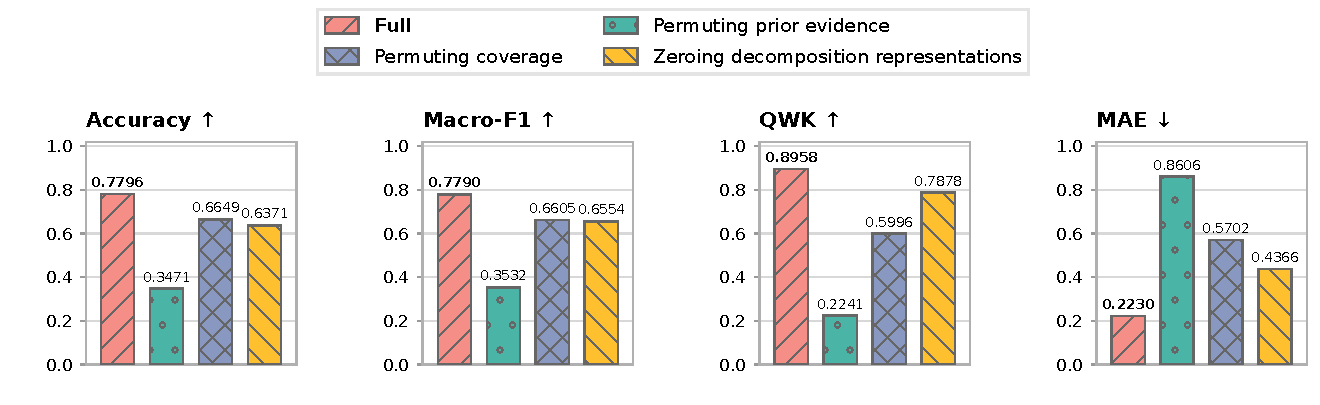
\includegraphics[width=\textwidth]{pic/ablation/pipeline_stages.pdf}
\caption{Pipeline-stage ablations on IdeaDelta. Full is the unablated checkpoint
of Table~\ref{tab:main}; each intervention is applied at inference without
retraining. Arrows indicate the preferred direction for each metric.}
\label{fig:ablation-pipeline}
\end{figure}

\begin{figure}[t]
\centering
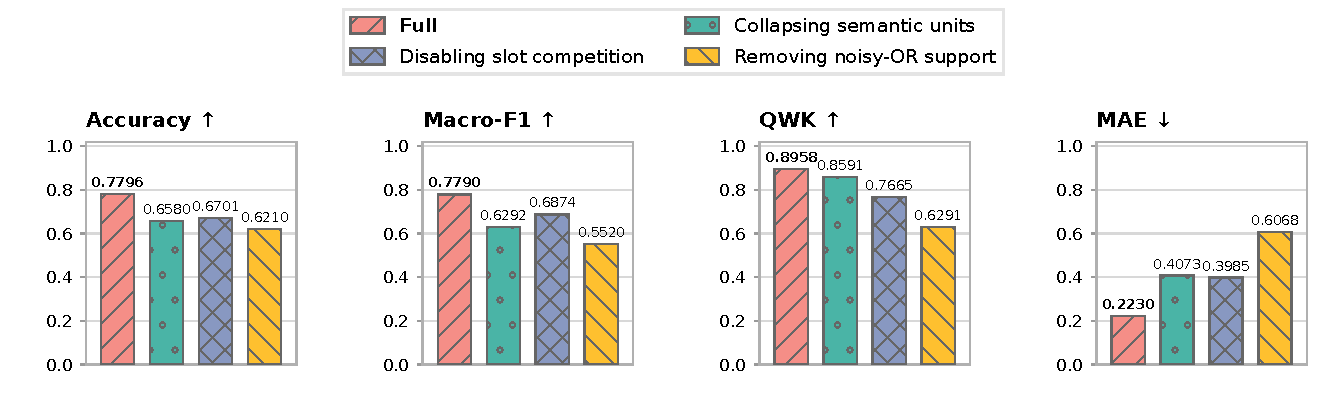
\includegraphics[width=\textwidth]{pic/ablation/decomposition_design.pdf}
\caption{Decomposition-design ablations on IdeaDelta. Each variant is retrained
without the corresponding component and compared with the same Full model.
Arrows indicate the preferred direction for each metric.}
\label{fig:ablation-decomposition}
\end{figure}

Because the supplied evidence can be intervened on with the target held fixed,
we can test what the trained model's predictions actually depend on. The three
pipeline interventions in Figure~\ref{fig:ablation-pipeline} cut the chain at
successive points.
\textbf{Permuting prior evidence} shuffles the retrieved prior texts across
targets, breaking the correspondence between each target and its evidence in
Stage~A. \textbf{Permuting coverage} shuffles only the joint coverage score
produced by Stage~A while leaving every prior text in place.
\textbf{Zeroing decomposition representations} sets the unit residual $\boldsymbol{z}_U$,
interaction residual $\boldsymbol{z}_I$ and covered-content representation
$\boldsymbol{z}_C$ to zero, removing these three outputs of Stage~B
together. All three reduce performance on
every metric.

Permuting prior evidence causes the largest loss across all four metrics,
establishing target--prior correspondence as a critical basis for the model's
predictions. Permuting coverage preserves the prior texts but sharply reduces
ordinal agreement and increases grade errors, showing that the remaining inputs
cannot compensate for a corrupted coverage signal. Zeroing decomposition
representations produces more incorrect predictions than permuting coverage,
but smaller grade errors on average. Together, these
results suggest complementary roles for coverage in maintaining ordinal
agreement and decomposition representations in assigning the exact grade.

Figure~\ref{fig:ablation-decomposition} shows that the three mechanisms inside
the decomposition are not interchangeable; each removal degrades a different
part of the prediction.
\textbf{Collapsing semantic units} from eight to one costs on Accuracy, Macro-F1
and MAE while QWK barely moves.
\textbf{Disabling slot competition}, which removes the softmax through which the
units compete for each token, reverses that pattern: QWK falls while MAE stays
where collapsing the units left it.
\textbf{Removing noisy-OR support} costs the most of the three on all four
metrics and most of all on the rank-sensitive ones.

We also conduct parameter sensitivity experiments using the default configuration,
with detailed results reported in
Appendix~\ref{app:sensitivity}.

\subsection{Case study}
\label{sec:exp-case}

% Figure: figures/case_study/make_figure.py, from figures/case_study/pull_full.npz
% and figures/case_study/cases.json. Cases CI_26954 (low), CI_18669 (moderate),
% CI_18985 (high); every number below is read off those two artifacts.
\begin{figure}[t]
\centering
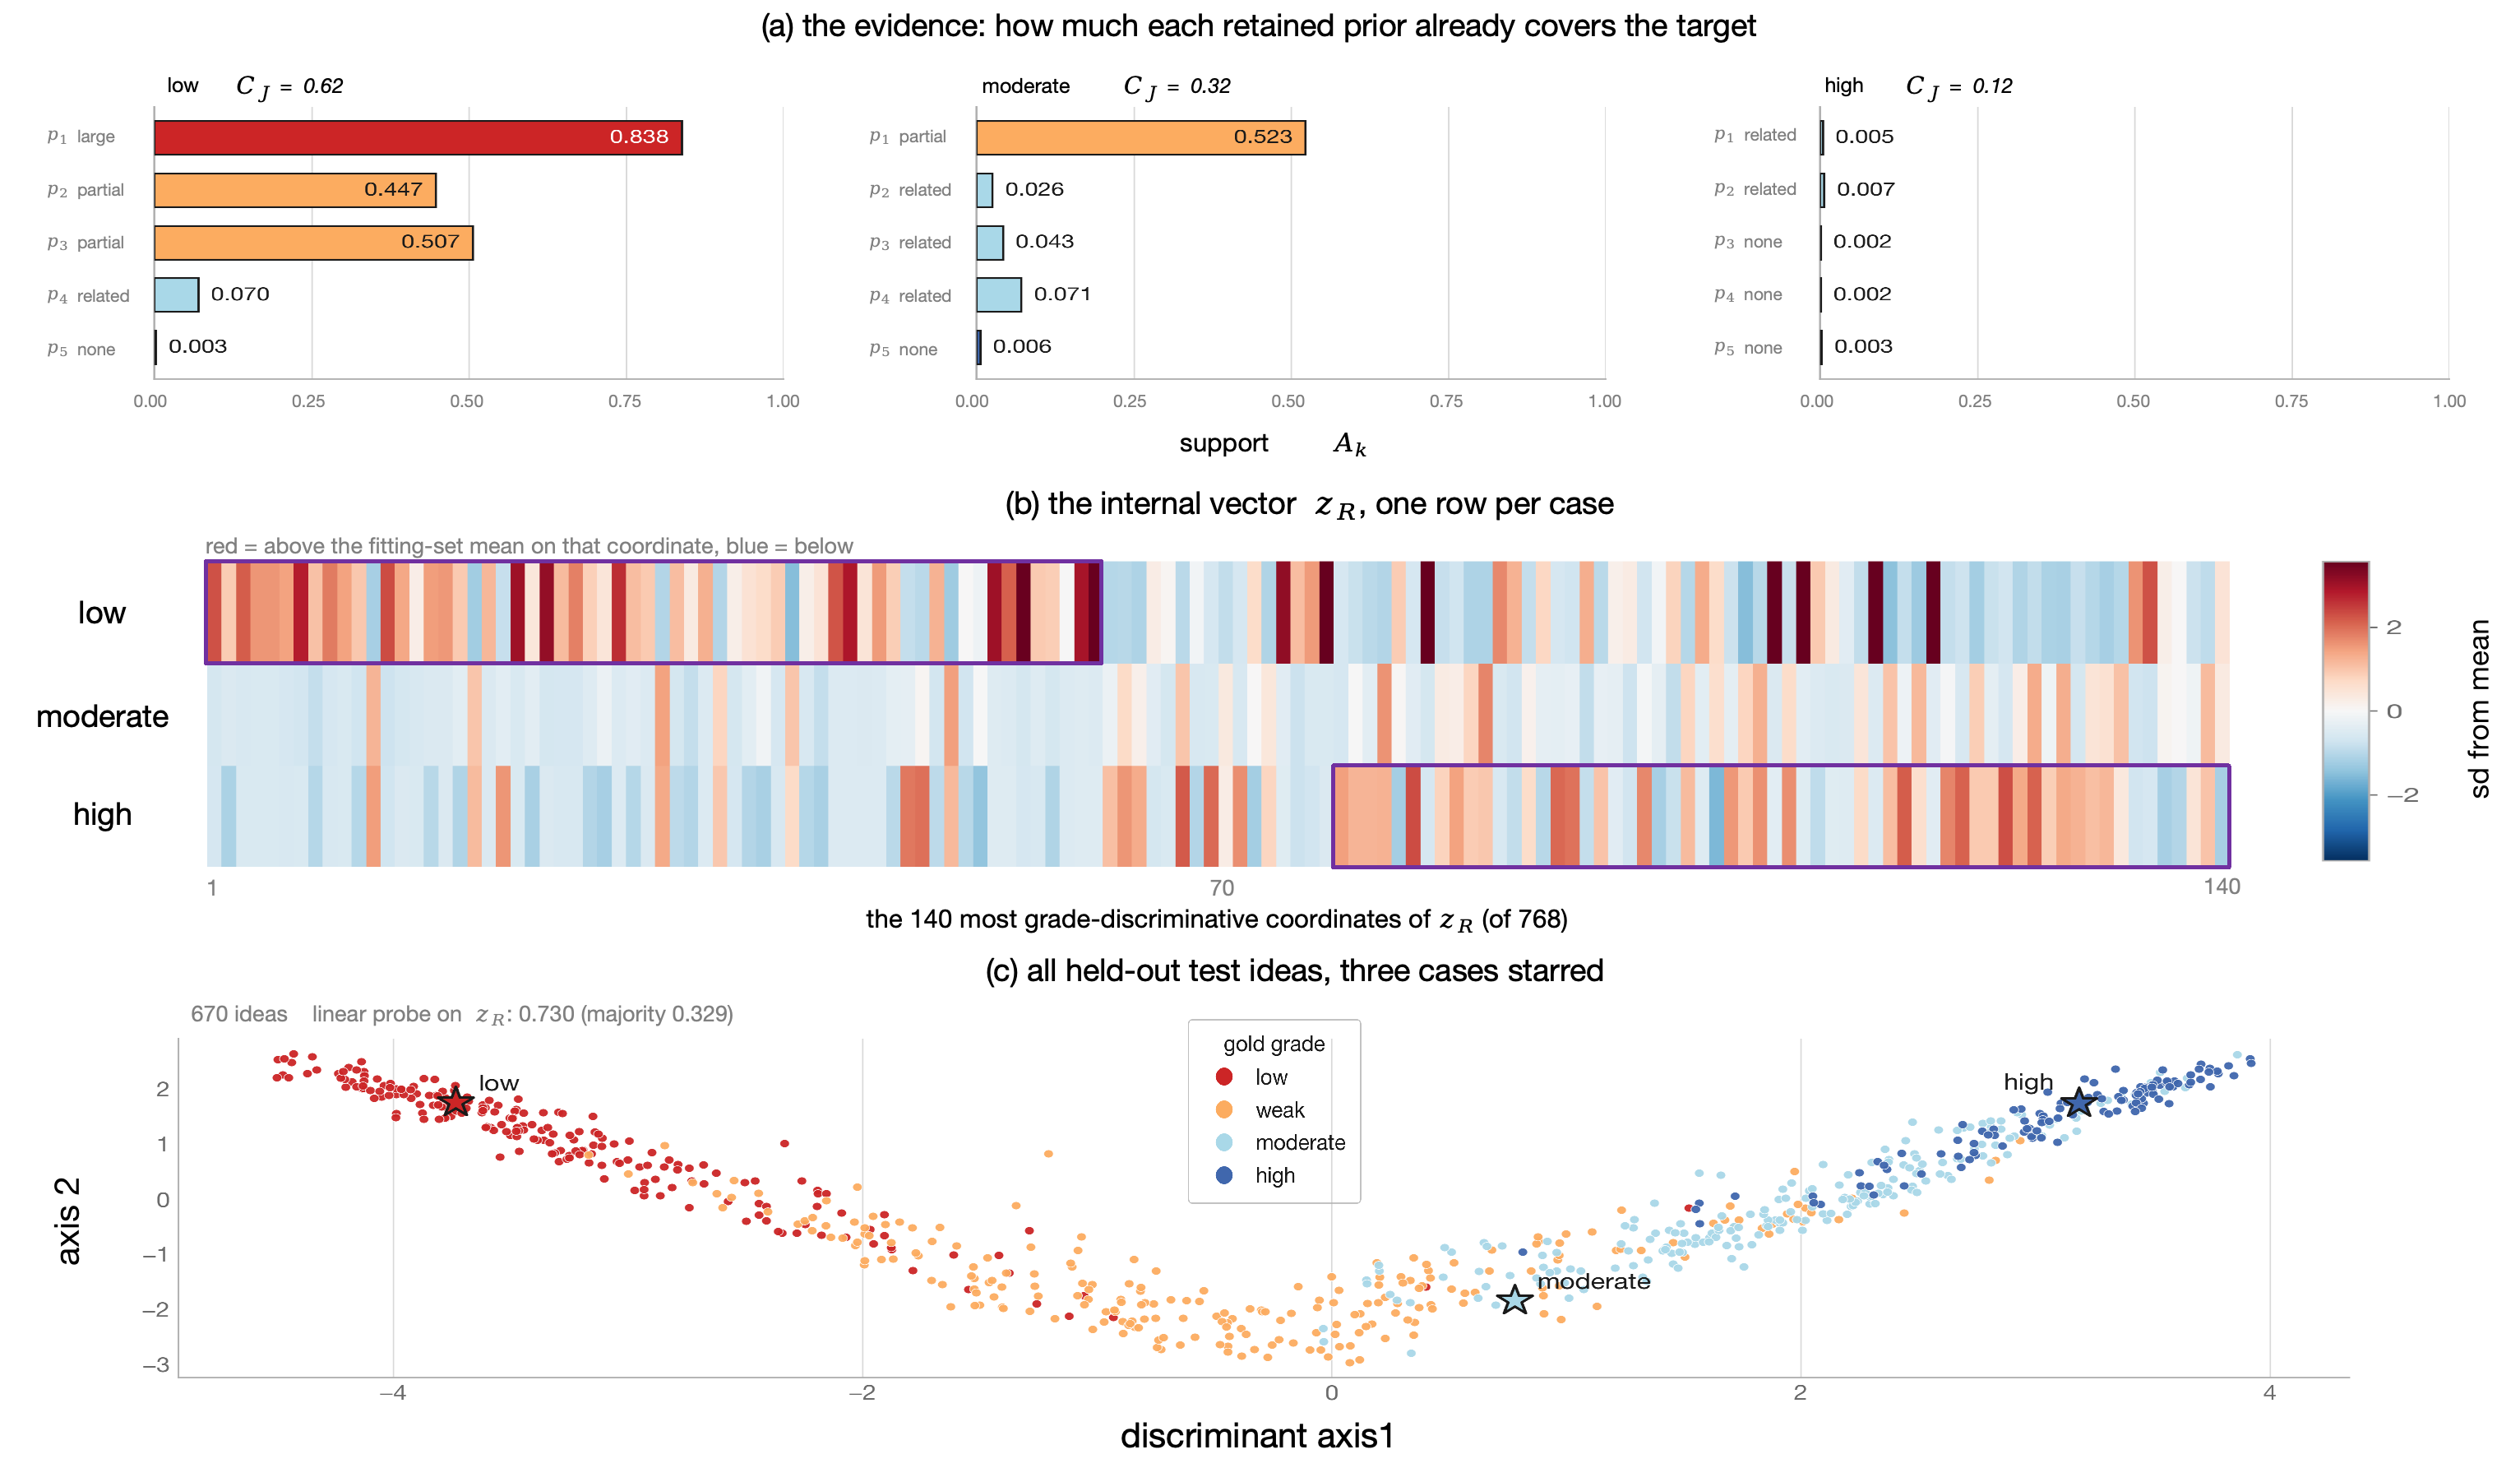
\includegraphics[width=\textwidth]{pic/case_study.png}
\caption{Three test targets, graded low, moderate and high, traced through the
model. \textbf{(a)} The support $A_k$ assigned to each retained prior, against
the coverage label the annotation carries; $C_J$ is the predicted joint
coverage. \textbf{(b)} The residual representation $\boldsymbol{z}_R$ of each
case, as deviations from the fitting-set mean. \textbf{(c)} $\boldsymbol{z}_R$ for
every held-out test idea, coloured by gold grade, the three cases starred.}
\label{fig:case-study}
\end{figure}

Figure~\ref{fig:case-study} traces three correctly predicted cases from
evidence coverage to residual representations. Joint coverage decreases from
the low- to the high-novelty case, while their residual embeddings show
distinct patterns. In the supervised discriminant projection, held-out ideas
are broadly ordered by novelty along the first axis, with overlap between
adjacent grades; the three cases occupy regions consistent with their labels.
These examples illustrate the association between evidence coverage and
novelty-sensitive representations. Appendix~\ref{app:case-study} provides
visualization details.
